\chapter{Results}\label{ch:results}

\section{Predicted and observed yields}\label{sec:results_yields}

Figure~\ref{fig:results_mj_dists} shows the predicted and observed $M_J^{\Sigma}$ distributions in the four-jet and five-jet regions, along with the total estimated uncertainty.
The red solid line indicates the estimated yield in each $M_J^{\Sigma}$ bin, and the red shaded area shows the total uncertainty, including statistical and systematic uncertainties.
The gray dashed lines are the $\pm1\sigma$ bands from the statistical uncertainty only.
There is good agreement between predicted and observed event yields across a range of $\pm1\sigma$ values, within the total uncertainty.
The exception is in the five-jet signal region, where a slight excess of events is observed.
After statistical analysis, discussed in~\ref{sec:results_stats}, the excess is found to not be significant.
The $M_J^{\Sigma}$ distributions for two different cascade decay signal mass points are also shown on the plots, to visualize the effect that the existence of signal events would hve on the distributions.

\begin{figure}[!ht]
    \centering
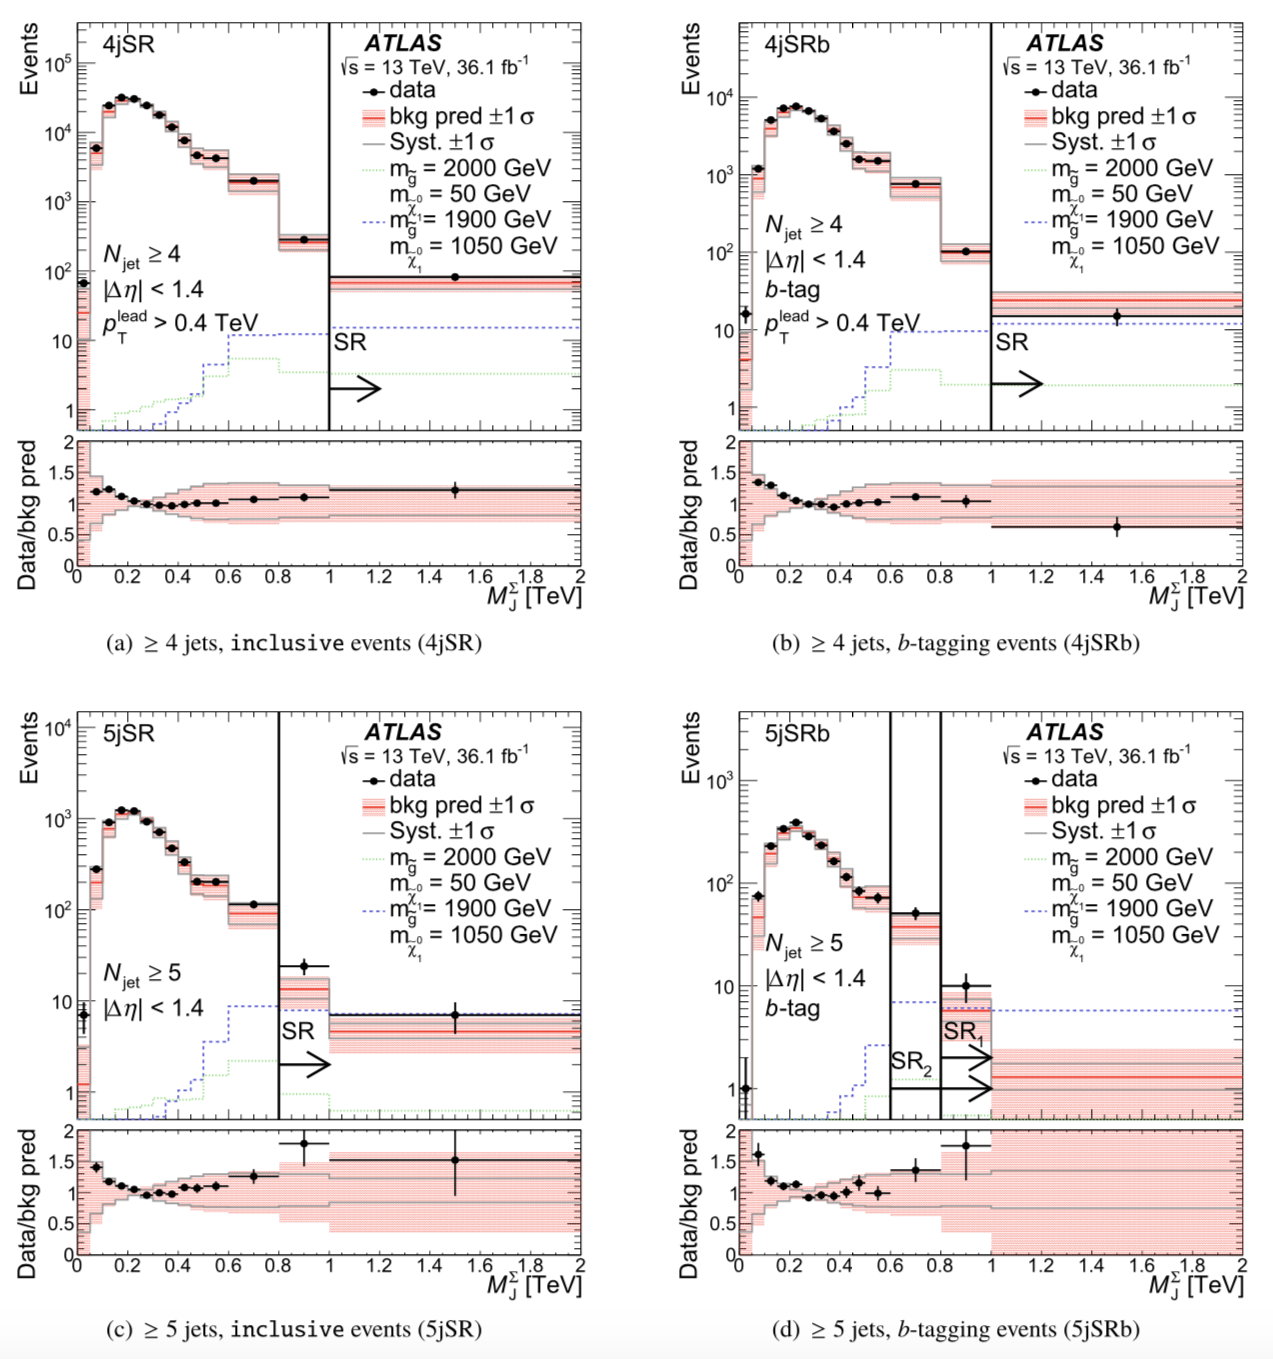
\includegraphics[width=0.8\linewidth]{results_mj_dists}
\caption{Distribution of $M_J^{\Sigma}$ in the four-jet inclusive (4jSR), four-jet b-tag (4jSRb), five-jet inclusive
(5jSR), and five-jet b-tag (5jSRb) regions.
The solid red lines show the predicted $M_J^{\Sigma}$ distributions, along with the total uncertainty shaded in red.
The black dots show the observed $M_J^{\Sigma}$ distributions.
The corresponding $M_J^{\Sigma}$ cuts are indicated with the solid black vertical line and arrow for each region.
Two separate signal regions are defined for the 5jSRb region, one with an $M_J^{\Sigma}$ cut of $0.6~TeV$,
and one with a cut of $0.8~TeV$.
The green and blue dashed lines show the predicted $M_J^{\Sigma}$ contribution from cascade-decay signal events
from two different mass points.
}
\label{fig:results_mj_dists}
\end{figure}

In the four-jet signal regions, no excess of events was observed.
In the five-jet signal regions, an excess of events were observed, but these excesses were not found to be statistically significant.
Predicted and observed yields in all signal regions are shown in table~\ref{tbl:results_yields_table}, including the number of events in the corresponding normalization region, $N_{NR}$, and the statistical and systematic uncertainties on the background yield predictions in those regions.
Table~\ref{tbl:results_yields_table} also shows the number of events in the normalization region, $N_{NR}$, corresponding to each signal region.
The central value of the prediction for each signal region is shown, as well as the statistical uncertainty, and the systematic uncertainties from the low-$p_T$ and high-$p_T$ uncertainty determination regions.

\begin{table}[!ht]
    \centering

    \begin{tabular}{lllrlllrlll}
        \toprule
        Region & $N_{NR}$ & $\geq M_{J}^{\Sigma}~[TeV]$ & Expected ( & $\pm$ & (stat.) & $\pm$ & (high-$p_T$) & $\pm$ & (low-$p_T$)) & Observed \\
        \midrule
        4jSRb     & 64081    & 1.0                       & 23.6       & $\pm$ & 4.6     & $\pm$ & 6.1          & $\pm$ & 1.7          & 15 \\
        4jSR      & 224862   & 1.0                       & 82.0       & $\pm$ & 7.6     & $\pm$ & 15.8         & $\pm$ & 4.4          & 82 \\
        5jSRb$_1$ & 2177     & 0.8                       & 7.0        & $\pm$ & 2.4     & $\pm$ & 1.9          & $\pm$ & 0.7          & 10 \\
        5jSRb$_2$ & 2177     & 0.6                       & 44.0       & $\pm$ & 7.5     & $\pm$ & 11.2         & $\pm$ & 7.2          & 61 \\
        5jSR      & 6592     & 0.8                       & 18.0       & $\pm$ & 3.7     & $\pm$ & 4.6          & $\pm$ & 1.5          & 31 \\
        \bottomrule
    \end{tabular}

\caption{Predicted and observed yields in all signal regions used in the analysis.
The number of events in the corresponding normalization regions, $N_{NR}$ is shown.
For each signal region, the minimum value of $M_J^{\Sigma}$ used to define that region is also shown.
Additionally, the statistical uncertainty on the background yield, as well as the two systematic uncertainties,
derived from the high-$p_T$ and low-$p_T$ UDRs are shown~\cite{paper-plb}.}
\label{tbl:results_yields_table}
\end{table}

\section{Statistical Interpretation}\label{sec:results_stats}

The data are interpreted in a frequentist framework by defining a likelihood-ratio test statistic, and calculating a $p$-value under the null hypothesis that no signal is present.
If the hypothesis cannot be rejected, then there is no evidence for the signal process, and limits can be set on the signal production cross section.
The limit-setting procedure uses the $\text{CL}_s$ method~\cite{results-stats-asymptotic,results-stats-cls}.
The likelihood function for an observed yield $k$ and expected yield $\lambda$ is:
\begin{equation}
    L(\mu) = P(k|\lambda)\Product_{l}G(0|\theta_{l}, 1)
\end{equation}
where $\mu$ is a signal-strength parameter, $P(k|\lambda)$ is the Poisson distribution with mean $\lambda$, and $G(0|\theta_{l}, 1)$ is a log-normal constraint term for systematic $l$.
Uncertainties are incorporated into the likelihood function as nuisance parameters, by parameterizing the expected yield as:
\begin{equation}
    \lambda = \mu\prod_{i}(1+\theta_i \sigma_i)S_0 +B_{0}\prod_j (1+\sigma_{b,j}\sigma_{b,j}) - \mu\Delta b (1+\theta_{b,stat}\sigma_{b,stat})
\end{equation}
where $\theta_i$ is the nuisance parameter for signal systematic $i$ with size $\sigma_i$, and $\theta_{b,j}$ is the nuisance parameter for background systematic $j$ with size $\sigma_{b,j}$.
Recall that each nuisance parameter is constrained by a log-normal constraint in the likelihood function.
$S_0$ is the nominal signal yield, and $B_0$ is the predicted background yield.
As described in~\ref{sec:signal_contamination}, the presence of signal contamination in the control region can increase the expected background prediction.
To correct for this, the signal contamination contribution to the background prediction must be subtracted off from the total expected yield $\lambda$.
This contribution is proportional to the signal strength, and is subject to statistical, but not systematic uncertainties.
So the term used to correct for signal contamination is $-\mu\Delta b(1+\theta_{b,stat}\sigma_{b,stat})$.

The test statistic $q_{\mu}$ is a ratio of two different likelihood function fits:
\begin{equation}
    q_{\mu} = -2\ln \frac{L(\mu, \hat{\theta})}{L(\hat{\mu}, \hat{\hat{\theta}})}
\end{equation}
where $\hat{\theta}$ are the best-fit values of the parameters when the likelihood function is fit to data with the signal-strength parameter $\mu$ kept fixed to the value of the null hypothesis,
and $\hat{\hat{\theta}}$ are the best-fit values of the parameters when $\mu$ is allowed to vary in the fit, along with the other parameters.

To test for evidence of the signal process, a hypothesis test is conducted with the null hypothesis that $\mu=0$, meaning that the signal process does not exist.
The frequentist interpretation of a $p$-value is the probability of observing an excess at least as large as what was seen in the data, assuming that the signal process does not exist.
A $p$-value of $3\times10^{-7}$ or less is required to reject the null hypothesis.
The $p$-value threshold is equivalent to the false-positive rate, so the probability of incorrectly rejecting the null hypothesis due to a statistical fluctuation will be $3\times10^{-7}$ for this test.
A separate $p$-value is calculated for each of the signal regions.
The $p$-values for each of the signal regions can be seen in table~\ref{tbl:results_model_ind_limits}.
None of the $p$-values are below the threshold, so no evidence of the signal process was found.

\begin{table}[!ht]
    \centering

    \begin{tabular}{lllll}
        \toprule
        Signal Region & $M_{J}^{\Sigma}$ requirement & Expected limit $[fb]$  & Observed limit $[fb]$ & $p_0$-value \\
        \midrule
        4jSRb           & $>1.0~TeV$                      & $0.53^{+0.20}_{-0.12}$ & 0.37 & 0.5   \\
        4jSR            & $>1.0~TeV$                      & $1.12^{+0.50}_{-0.32}$ & 1.50 & 0.24  \\
        5jSRb$_1$       & $>0.8~TeV$                      & $0.24^{+0.10}_{-0.06}$ & 0.34 & 0.26  \\
        5jSRb$_2$       & $>0.6~TeV$                      & $0.86^{+0.40}_{-0.20}$ & 1.32 & 0.20  \\
        5jSR            & $>0.8~TeV$                      & $0.44^{+0.18}_{-0.10}$ & 0.84 & 0.062 \\
        \bottomrule
    \end{tabular}

    \caption{Observed and expected limits on gluino pair-production cross section for each of the signal regions,
    along with the p-value for any excess observed in each region~\cite{paper-plb}.}
\label{tbl:results_model_ind_limits}
\end{table}

Using the observed yields, upper bounds can be set on the cross-section of the two signal models, as well as model-independent upper bounds.
The same test statistic can be used in the limit-setting procedure as was used in the discovery test.
In this case, the signal strength parameter $\mu$ will be fixed to 1 in the numerator of the likelihood-ratio.
This corresponds to a null hypothesis of a signal process existing with cross-section equal to the theoretical prediction.
For a given signal point, if the $p$-value falls below 0.05, the signal plus background hypothesis will be rejected, and that point will be considered excluded.
Since signal yields are only determined at discrete mass points, the limits are smoothly interpolated between points.

The resulting limits for the cascade decay scenario are shown in figure~\ref{fig:results_ten_quark_limits}.
The observed limit and its theoretical uncertainty are shown in red, and the expected limit is shown in black with 1 sigma band shown in yellow.
For comparison, the limits set by the Run-1 analysis are shown in gray.
The result is a significant increase in the excluded parameter space for this model.
The gluino mass excluded varies from $1~TeV$ to $1.875~TeV$ depending on the value of $m_{tilde{\chi}_1^0}$.

\begin{figure}[!ht]
    \centering
    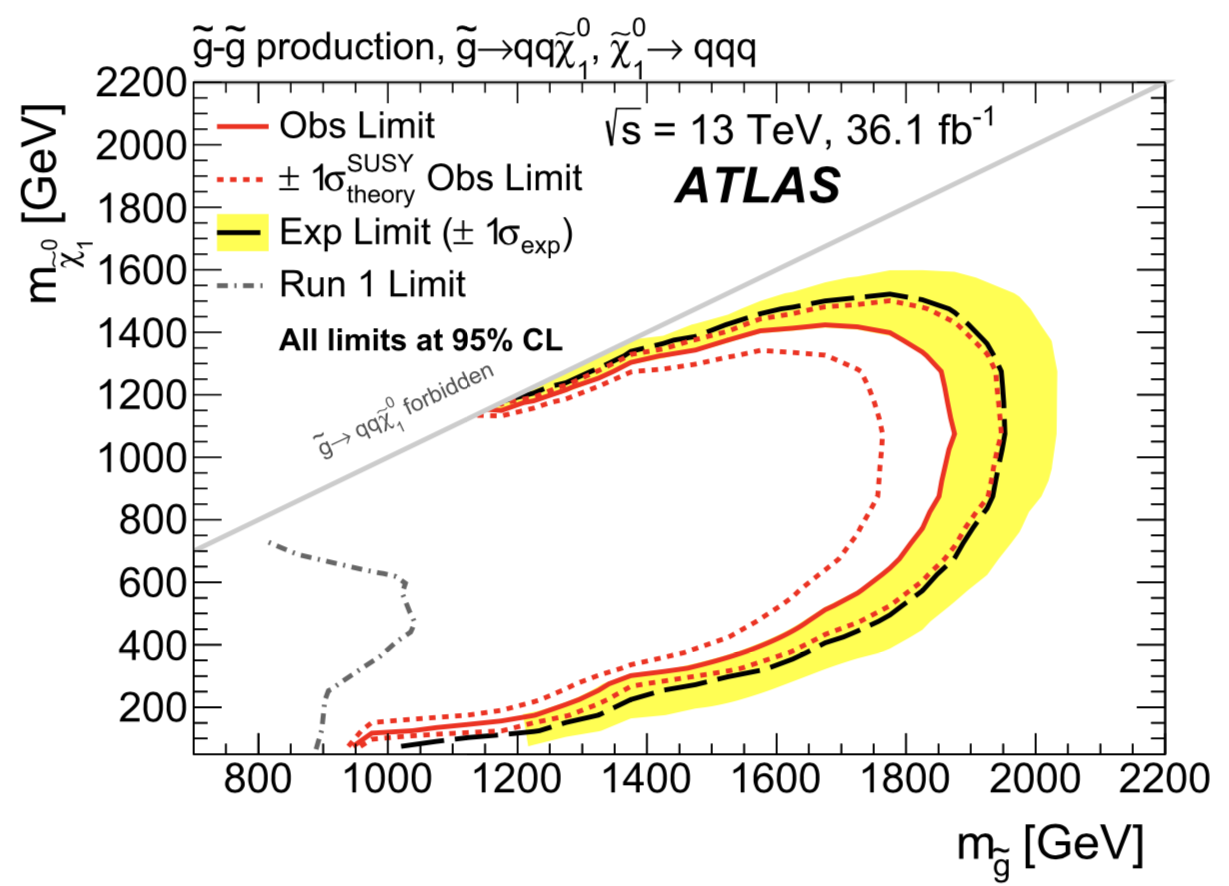
\includegraphics[width=0.8\linewidth]{results_ten_quark_limits}
    \caption{Predicted and observed limits for the cascade decay model over a range of $m_{\tilde{g}}$ and $m_{\tilde{\chi}_1^0}$ values.
    Both predicted and observed limits are shown with $1\sigma$ uncertainty bands.
    The gray dashed curve shows the limits from the Run-1 analysis.
    Due to slight excess in the signal region, the observed limit is less than expected~\cite{paper-plb}.}
\label{fig:results_ten_quark_limits}
\end{figure}

For the direct decay scenario, a similar limit-setting method was used, with $p$-values calculated over a range of gluino masses and also over a range of $\mu$ values.
For a given gluino mass and value of $\mu$, if the $p$-value is less than 0.05, the gluinos with that mass and production cross-section are considered excluded.
This allows for lower bounds to be placed on the gluino cross-section over a range of gluino mass values.

The resulting limits for the direct-decay model are shown in figure~\ref{fig:results_six_quark_limits}.
The theoretical $\tilde{g}\tilde{g}$ production cross-section as a function of $m_{\tilde{g}}$ is shown as a red dashed line, with gray band indicating the uncertainty.
The expected limit is shown as a black dashed line with green and yellow bands indicating the one- and two-sigma uncertainty extent, and the observed limit is a solid black line.
Because of the small excess of events observed in the signal region, the upper bound on the production cross section is higher than the theoretical production cross section in the entire gluino mass range that was tested, from $900~GeV$ to $1.8~TeV$.
So no new limits can be set on the mass of the gluino decaying through this channel.

\begin{figure}[!ht]
    \centering
    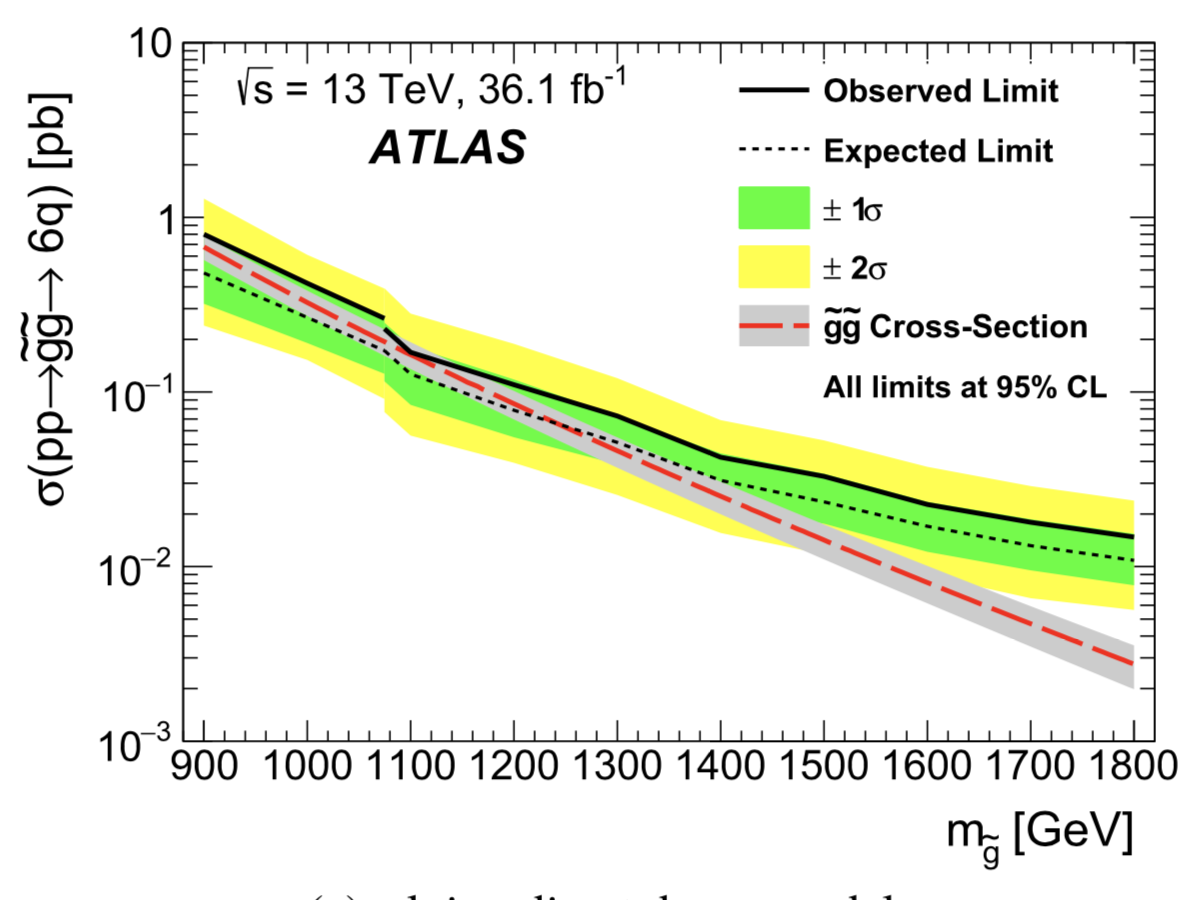
\includegraphics[width=0.8\linewidth]{results_six_quark_limits}
    \caption{Predicted and observed cross-section limits for the direct decay model over a range of $m_{\tilde{g}}$ values.
    Also shown are the estimated gluino pair production cross-sections at each mass point~\cite{paper-plb}.}
\label{fig:results_six_quark_limits}
\end{figure}
